\subsection{Adeline}

\begin{frame}
\frametitle{\underline{ADA}ptive \underline{LIN}ear \underline{E}lement}

\comment{
\begin{itemize}
\item \textbf{ADA}ptive \textbf{LIN}ear \textbf{E}lement
\item Verzicht auf die Einheits-Sprungfunktion 
\item Stattdessen Nutzung linearer Aktivierungsfunktion 
\begin{itemize}
	\item wird erst einmal mit der Identiätsfunktion bestzt
\end{itemize}
\item Klassifizierungs- bzw. Entscheidungsfunktion im letzten Schritt
\begin{itemize}
	\item irrelevant für Trainingsalgorithmus
\end{itemize}
\end{itemize}
}

\begin{figure}
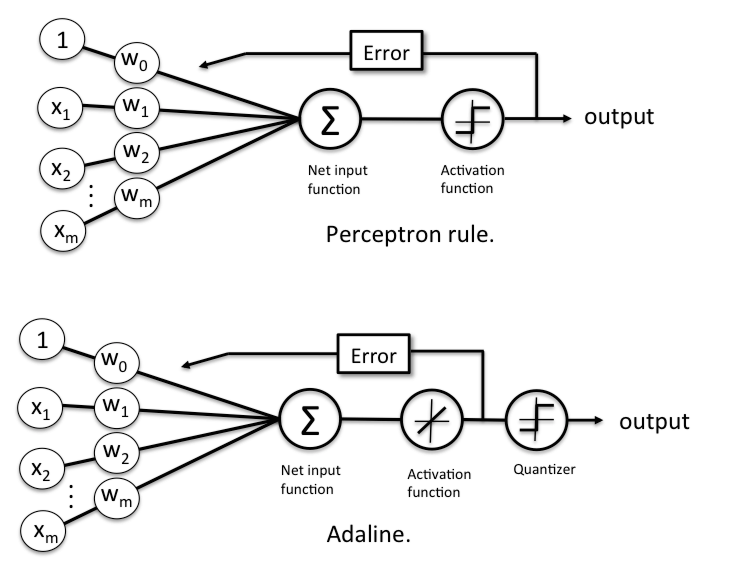
\includegraphics[width=.9\linewidth]{./geschichtliches/adeline/img/adeline_aufbau}
\end{figure}

\note[item]{1959: Stanford Prof. Bernard Widrow \& Elektroingenieur Marcian Edward Hoff}
\note[item]{ADELINE: ADAptive LINear Element}
\note[item]{Modell: Verzicht auf Einheitssprungfunktion bei Angleichung der Gewichte
\begin{itemize}
    \item Stattdessen lineare Aktierungsfunktion 
    \item erstmal nur Identitätsfunktion verwendet
    \item Entscheidungsfunktion für output weiterhin verwendet
\end{itemize}}

\end{frame}


\begin{frame}
\frametitle{Delta-Regel}

\begin{itemize}
\item Leralgorithmus durch Erfinder geprägt
\item auch unter \emph{Least-Mean-Square}-Algrithmus bekannt
\item Wesentlicher Vorteil: Ableitbare Kostenfunktion
\end{itemize}

\hspace{2mm}

\begin{block}{Notation}
\begin{align*}
J(w)  = \frac{1}{2} \sum_{i} (\text{target}^{(i)} - \text{output}^{(i)})^2 \quad \quad \text{output}^{(i)} \in \mathbb{R} \\
\end{align*}
\end{block}


\note[item]{Auch unter \emph{Least-Mean-Square-Algorithmus} bzw. \emph{Regressionsquadratsumme} bekannt
\begin{itemize}
    \item noch heute relevant
\end{itemize}}

\note[item]{Funktion stellt Kostenfunktion dar
\begin{itemize}
    \item Fehler bei Kostenfunktion soll mithilfe der Lernregel minimiert werden
\end{itemize}}

\note[item]{Vorteil dieses Ansatzes: Ableitbare Kostenfunktion}
\note[item]{Formel erläutern:
\begin{itemize}
    \item Differenz quadriert um Vorzeichen zu verlieren
    \item Faktor 1 / 2 vorschieben um Ableitung einfacher zu gestalten
    \item über alle Trainingsdatensätze der Menge iterieren
    \begin{itemize}
        \item Größe i
    \end{itemize}
\end{itemize}}

\note[item]{Für genaueres Verständnis erstmal Einschub mit Gradientenverfahren}

\end{frame}



\begin{frame}
\frametitle{Gradientenverfahren}

\hspace{1.5mm}

\begin{itemize}
\item Ziel: Gradientenvektor für bestimmten Input bestimmen: $\nabla J \equiv \left(\frac{\partial J}{\partial w_1}, \ldots, \frac{\partial J}{\partial w_m}\right)^T.$
\end{itemize}


\begin{figure}
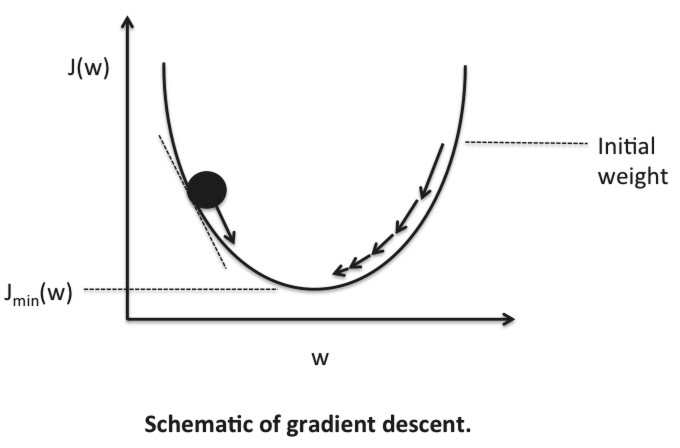
\includegraphics[width=.8\linewidth]{./geschichtliches/adeline/img/adeline_gd1_alpha}
\end{figure}


\note[item]{Wesentlicher Nachteil der Sprungfunktion: Nicht stetig \& damit nicht differenzierbar}
\note[item]{Adeline verwendet Identitätsfunktion}
\note[item]{Abbildung erläutern, Metapher: Ball rollt Hügel herunter
\begin{itemize}
    \item Abbildung erstmal nur mit einem einzelnen Gewicht geplottet
    \item Ableitung an einer bestimmten Stelle gleich der Steigung
    \item Gradientenvektor gibt diese Richtung an
    \begin{itemize}
        \item Mehrdimensional wenn mehreren Eingabeargumenten vorhanden
    \end{itemize}
    \item Steigung muss invertiert werden
\end{itemize}}

\note[item]{Es folgt: Exkurs - Partielle Ableitungen}

\end{frame}


\begin{frame}
\frametitle{Partielle Ableitungen}

\begin{columns}

\column{0.5\textwidth}
\begin{itemize}
\item Differenzieren von Funktionen mit mehreren Eingabewerten
\item Beispiel: $z = f(x) = x^2 + y^2$
\end{itemize}

\hspace{2mm}

\begin{block}{Partielle Ableitung - Notation}
\begin{align*}
\frac{\partial Abzuleitende Fkt.}{\partial Betrachtete Komponente}
\end{align*}
\end{block}

\column{0.5\textwidth}
\begin{figure}
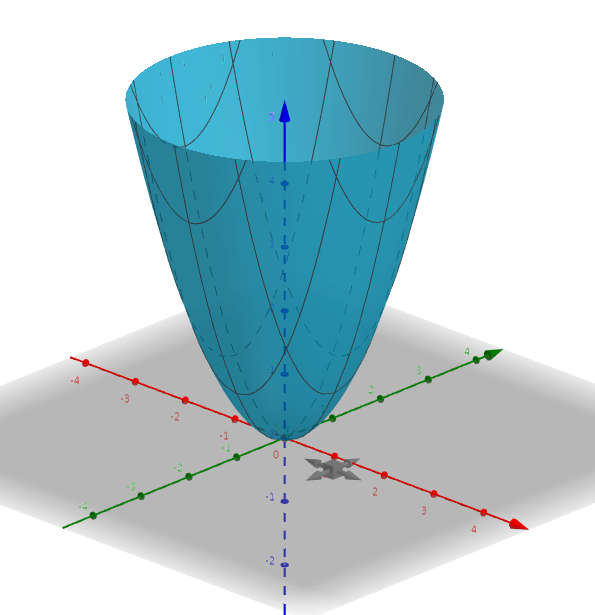
\includegraphics[width=\linewidth]{./geschichtliches/adeline/img/partAbl_1_alpha}
\end{figure}

\end{columns}


\note[item]{Notation: Bruch
\begin{itemize}
    \item Zähler: Abzuleitende Funktion
    \item Nenner: Betrachtete Komponente 
\end{itemize}}

\note[item]{Abbildung: Fkt. geplottet mit 2 Eingabekomponenten
\begin{itemize}
    \item Funktion: $z = f(x) = x^2 + y^2$
    \item Metapher: Blickwinkel erläutern
    \item nächste Folie miteinbeziehen
\end{itemize}}

\end{frame}


\begin{frame}
%\frametitle{Partielle Ableitungen}

\begin{columns}
\column{0.65\textwidth}
\begin{figure}
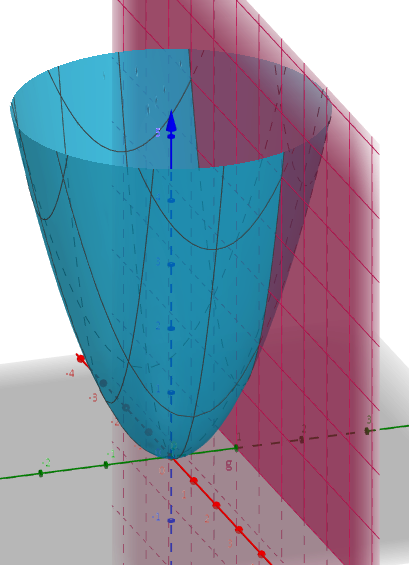
\includegraphics[width=.78\linewidth]{./geschichtliches/adeline/img/partAbl_2_alpha}
\end{figure}

\column{0.45\textwidth}
\begin{figure}
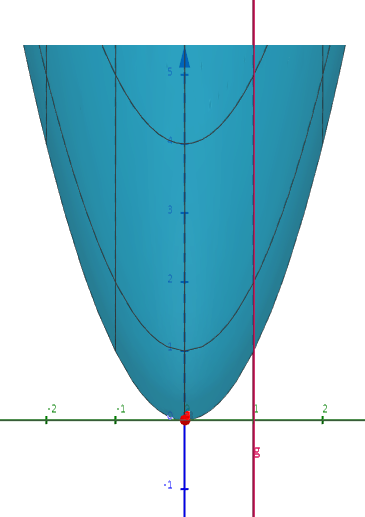
\includegraphics[width=.6\linewidth]{./geschichtliches/adeline/img/partAbl_3_alpha}
\end{figure}

\begin{block}{Ableitung - Beispiel}
\begin{align*}
\begin{aligned}
& z = f(x, y) = x^2 + y^2 \\
& \frac{\partial z}{\partial x} = 2x \;\;\;\;\; \frac{\partial z}{\partial y} = 2y 
\end{aligned}
\end{align*}
\end{block}

\end{columns}

\note[item]{Metapher: Blickwinkel erläutern}

\end{frame}


\begin{frame}
\frametitle{Gradientenverfahren}

\begin{figure}
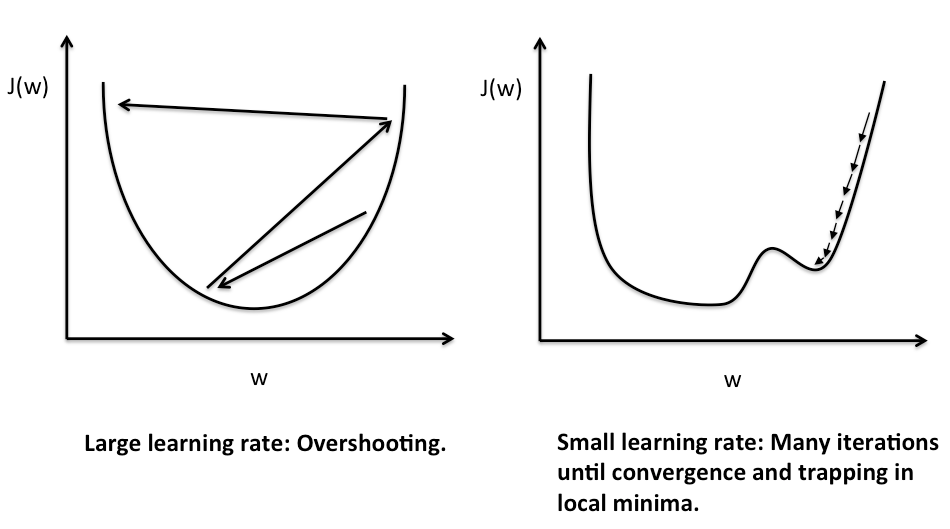
\includegraphics[width=\linewidth]{./geschichtliches/adeline/img/adeline_learning_rate_alpha}
\end{figure}

\note[item]{Lernrate kann als Schrittweite verstanden werden}
\note[item]{Zwei mögliche Probleme:
\begin{itemize}
    \item Overshooting: Schrittweite zu groß - Minimum wird nicht erkannt
    \item Lokales Minimum wird gefunden - Globales bleibt unerkannt
\end{itemize}}
\note[item]{Gradientenabstieg bisher nur in 2 Dimensionen (siehe nächste Folie}

\end{frame}


\begin{frame}
\frametitle{Gradientenverfahren}
\begin{figure}
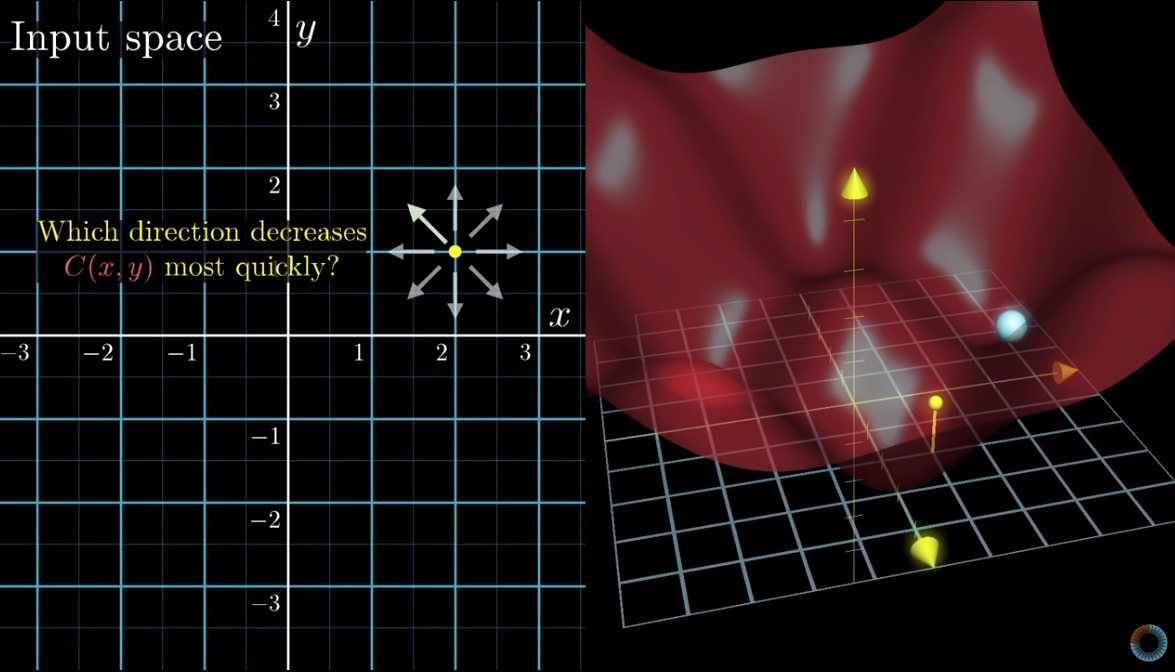
\includegraphics[width=\linewidth]{./geschichtliches/adeline/img/3dPlot_1}
\end{figure}

\note[item]{Abbildung: Gradientenabstieg in 3 Dimensionen geplottet}
\note[item]{Hier Ball-Metapher dargestellt}
\note[item]{Es folgt kompletter Durchlauf des Gradientenabsiegs}

\end{frame}


\begin{frame}
\frametitle{Gradientenverfahren}
\begin{figure}
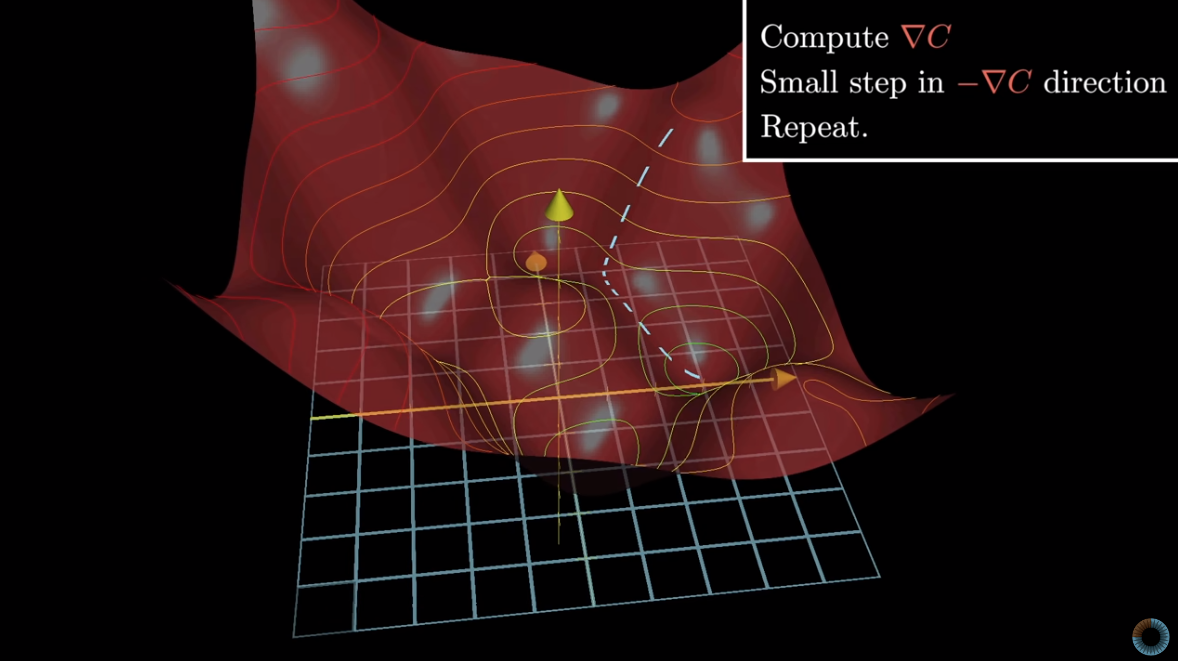
\includegraphics[width=\linewidth]{./geschichtliches/adeline/img/3dPlot_2}
\end{figure}

\note[item]{Abbildung: Gradientenabstieg in 3 Dimensionen geplottet}
\note[item]{Hier durchgeführter Gradientenabstieg}

\end{frame}


\begin{frame}
\frametitle{Gradientenverfahren}

\begin{block}{Gradientenverfahren - Anwendung}

\begin{itemize}

\item Gradientenvektor
\begin{align*}
\nabla J \equiv \left(\frac{\partial J}{\partial w_1}, \ldots, \frac{\partial J}{\partial w_m}\right)^T.
\end{align*}

\item Allgemein: Vektorielle Darstellung
\begin{align*}
\Delta w = - \eta \nabla J(w)
\end{align*}

\comment{$
\!
\begin{aligned}[t]
\Delta w = - \eta \nabla J(w)
\end{aligned}
$}

\item Für die jeweiligen Gewichte: Komponentenweise Darstellung
\begin{align*}
\Delta w_j = - \eta \frac{\partial J}{\partial w_j}
\end{align*}
\end{itemize}
\end{block}


\begin{itemize}
\item Angleichung der Gewichte $w = w + \Delta w$
\end{itemize}

\note[item]{Gradientenvektor: Richtung des \emph{Abstiegs}
\begin{itemize}
    \item mit \emph{Nabla} dargestellt (Dreieck)
    \item kann auch mehrdimensional sein
\end{itemize}}

\note[item]{Vektorielle Darstellung
\begin{itemize}
    \item Eingabeparameter werden als Vektor verstanden
    \item mit Gradientenvektor und Negativer Lernrate verrechnet / multipliziert
\end{itemize}}

\note[item]{Komponentenweise Darstellung
\begin{itemize}
    \item negative Lernrate mit partieller Ableitung verrechnet
\end{itemize}}

\note[item]{Angleichung der Gewichte:
\begin{itemize}
    \item wie schon bei vorherigen Modellen
    \item Mathematische Darstellung: $w = w + \Delta w$
\end{itemize}}

\end{frame}



\begin{frame}
\frametitle{Kostenfunktion ableiten}

\begin{align*}
\frac{\partial J}{\partial w_j} & = \frac{\partial }{\partial w_j} \frac{1}{2} \sum_i  (t^{(i)} - o^{(i)})^2 \\
 & = \frac{1}{2} \sum_i \frac{\partial }{\partial w_j} (t^{(i)} - o^{(i)})^2 \\
 & = \frac{1}{2} \sum_i 2 (t^{(i)} - o^{(i)}) \frac{\partial }{\partial w_j} (t^{(i)} - o^{(i)}) \\
 & = \sum_i (t^{(i)} - o^{(i)}) \frac{\partial }{\partial w_j} \bigg(t^{(i)} - \sum_j w_j x^{(i)}_{j}\bigg) \\
 & = \sum_i  (t^{(i)} - o^{(i)})(-x^{(i)}_{j})
\end{align*}


\note[item]{Ableiten der bisher vorgestellten Kostenfuntion (Least-Mean-Square)}
\note[item]{Summe und Faktor vorziehen}
\note[item]{Kettenregel anwenden
\begin{itemize}
    \item äußere Ableitung bereits bestimmt (Vorfaktor 2)
    \item innere Ableitung steht noch aus
\end{itemize}}

\note[item]{Faktor 2 kann vorgezogen werden, wird mit 1/2 verrechnet}
\note[item]{Ursprüngliche Notation für die Ausgabe wird eingesetzt:
\begin{itemize}
    \item Ausgabe: $\sum_j w_j x^{(i)}_{j}$
\end{itemize}}

\note[item]{Summe aufgelöst
\begin{itemize}
    \item es wird nach $w_j$ abgeleitet
    \item alle Summanden in denen dieser Faktor nicht vorkommt entfallen
\end{itemize}}

\end{frame}

